\begin{usecase}{Schedule Prayer Times}
  \ucbasicinfo{High}{Regular}
  \ucshortdescription{The calendar is blocked and updated automatically according to the person's time zone prayer time.}
  \uctrigger{This usecase is triggered when the user clicks the prayer time feature button in the settings page in the app.}
  \ucactors{User}{None}
  \ucpreconditions{User must be logged into the system.}
  \ucrelationships{N/A}{N/A}{N/A}
  \ucinputsoutputs{
    \begin{itemize}
      \item \textbf{User's IP Address} (Source: User)
      \item \textbf{User's City} (Source: System)
    \end{itemize}
    }{
      \begin{itemize}
        \item \textbf{.mobileconfig file for subscription calendar} (Source: System)
        \item \textbf{Prayer Time Calendar} (Source: System)
    \end{itemize}
  }
  \ucmainflow{
    \begin{enumerate}
      \item User clicks the option to schedule prayer times.
            \ucinfo{The system sends a request to start the process of adding schedule prayer times to the backend, sends the IP Address.}
      \item A sheet is shown to the user to download the `.mobileconfig' file
            \ucinfo{The user clicks the `Begin Download' button to start it in a Safari WebView, with instructions on what to continue.}
      \item The user continues in the settings, opened automatically, to finish setting up the provisiong profile.
            \ucinfo{The provisioning profile adds a subscription calendar forr the prayer times of the user's city to their calendat account.}
    \end{enumerate}
  }
  \ucalternateflows{
    \begin{itemize}
      \item The user doesn't enable the scheduling prayer time.
    \end{itemize}
  }
  \ucexceptions{
    \begin{itemize}
      \item If there's a system error, display a relevant error message.
    \end{itemize}
  }
  \ucpostconditions{The system generates calendar with prayer time}
  \ucspecialrequirements{The system must show the calendar according to their city}
  \ucconclusion{User's prayer times are successfully scheduled.}
\end{usecase}

\begin{figure}[!h]
  \centering
  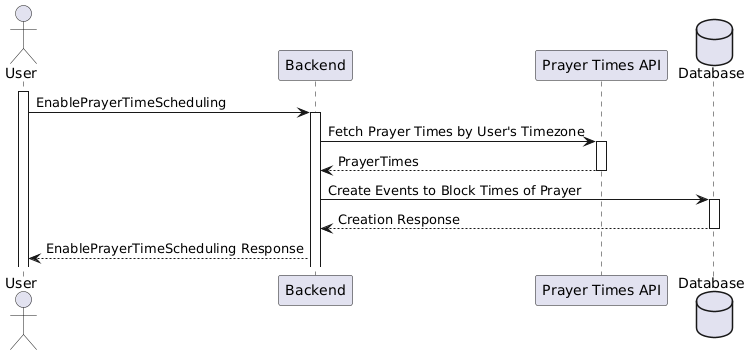
\includegraphics[width=\textwidth]{images/docs/diagrams/sequence-diagrams/all-sequence-diagrams/Schedule Prayer Times.png}
  \caption{Schedule Prayer Times Sequence Diagram}
  \label{fig:seq/schedule-prayer-times}
\end{figure}

The ``Schedule Prayer Times Sequence Diagram'', shown in \textbf{Figure~\ref{fig:seq/schedule-prayer-times}}, illustrates Jadwal's unique feature of automatically integrating prayer times into the user's device calendar via a subscription, based on their location. The process begins when the user clicks the option to add prayer times to the calendar within the app's settings.

Upon activation, the sequence follows these steps:
\begin{enumerate}
  \item The \textbf{User} taps the "Add Prayer Time Scheduling" option in the \textbf{App Frontend}.
  \item The \textbf{App Frontend} initiates the \texttt{SchedulePrayerTimes()} gRPC call to the \textbf{Backend}.
  \item The \textbf{Backend} determines the user's geographical location (e.g., using the IP address provided or other user information).
  \item The \textbf{Backend} queries the \textbf{Prayer Times API} using the determined location to fetch the relevant prayer times, receiving back a specific \textbf{iCal URL} that provides these times in a standard calendar format.
  \item The \textbf{Backend} returns the \texttt{iCalUrl} to the \textbf{App Frontend} in the \texttt{SchedulePrayerTimesResponse}.
  \item The \textbf{App Frontend} presents a sheet or prompt to the \textbf{User}, guiding them to download a \texttt{.mobileconfig} file. This configuration file is pre-filled with the received \texttt{iCalUrl}, setting up a calendar subscription.
  \item The \textbf{User} proceeds with the download and follows the device prompts (often involving the Settings app) to install the configuration profile, thereby subscribing their device's calendar to the provided iCal URL.
\end{enumerate}

This subscription-based process ensures that:
\begin{itemize}
  \item Prayer times are accurately sourced based on geographical location via the iCal feed.
  \item The user's device calendar automatically fetches and displays the prayer times, updating them as needed according to the subscription.
  \item Users can easily view their prayer schedule alongside other commitments within their standard calendar application.
\end{itemize}

The system's ability to facilitate this calendar subscription demonstrates Jadwal's commitment to supporting users' religious obligations seamlessly within their existing digital tools.
